%%%%%%%%%%%%%%%%%%%%%%%%% 
%% SITE A GARDER : http://titilog.free.fr/


\documentclass[10pt]{beamer}
% \includeonlyframes{yy}
\usepackage[french]{babel}
\usepackage{color, colortbl}
\definecolor{Gray}{gray}{0.9}
\newcolumntype{g}{>{\columncolor{Gray}}c}
\hypersetup{%
  % pdfborder = {0 0 0},
  colorlinks, urlcolor=blue, linkcolor=, }

\makeatletter \let\@mycite\@cite
\def\@cite#1#2{{\hypersetup{linkcolor=mLightBlue}[{#1\if@tempswa ,
      #2\fi}]}} \makeatother

\usetheme{m} %%%%%
% \usepackage[version=3]{mhchem}
\usepackage{caption}
\captionsetup[figure]{labelformat=empty}
\usepackage{fontspec}
\usepackage{xcolor}
\usepackage{siunitx}
% \usepackage[backend=bibtex]{biblatex} \usepackage[square]{natbib}
% \bibliography{main}
\usepackage[]{algorithm2e}
\usefonttheme[onlymath]{serif} \usepackage{amsmath}
\usepackage{appendixnumberbeamer}
\usepackage{tabularx, booktabs} \usepackage{multirow}
\usepackage{multicol} \usepackage{array} \usepackage{pbox}
\usepackage{mathtools}
\usepackage{adjustbox}
\definecolor{darkred}{HTML}{D38989}
\definecolor{darkgreen}{HTML}{66D191}
\PassOptionsToPackage{enumerate}{shortlabels} \newcommand\ExtraSep
{\dimexpr\cmidrulewidth\relax}
\captionsetup{font=scriptsize,labelfont=scriptsize}
% \addtobeamertemplate{background canvas}{\transfade[duration=0.05]}{}

\usepackage[skip=3pt]{subcaption}
\setlength{\belowcaptionskip}{2pt}
\newcommand{\rulesep}{\unskip\ \vrule\ }

\title{Fusion d'images IRM et MALDI en 3D}
\subtitle{Analyse statistique}

\author{{Florent \textsc{Grélard}\\
    David \textsc{Legland}, Mathieu \textsc{Fanuel}, Loïc \textsc{Foucat}, Hélène \textsc{Rogniaux}}} \titlegraphic{\hspace*{0.18\textwidth}~%
  
\includegraphics[width=0.26\textwidth]{fig/logo-inrae}\hspace*{0.18\textwidth}~%
  
\includegraphics[width=0.26\textwidth]{fig/logo-bibs.png}\hspace*{0.1\textwidth}~%
} \setbeamercolor{bbb}{fg=red}

\let\oldfootnotesize\footnotesize
\renewcommand*{\footnotesize}{\oldfootnotesize\tiny}
\newcommand\labelitemi{$\bullet$}
\renewcommand{\thefootnote}{[\arabic{footnote}]}
% \newrobustcmd*{\footlessfullcite}{\AtNextCite{\renewbibmacro{in:}{}\renewbibmacro{year:}{}}\footfullcite}
% \newrobustcmd*{\lessfullcite}{\AtNextCite{\renewbibmacro{in:}{}\renewbibmacro{year:}{}}\fullcite}

\newcommand{\cfbox}[2]{%
    \colorlet{currentcolor}{.}%
    {\color{#1}%
    \fbox{\color{currentcolor}#2}}%
}


\newcommand{\backupbegin}{ \newcounter{framenumberappendix}
  \setcounter{framenumberappendix}{\value{framenumber}} }
\newcommand{\backupend}{
  \addtocounter{framenumberappendix}{-\value{framenumber}}
  \addtocounter{framenumber}{\value{framenumberappendix}} }
% http://mcclinews.free.fr/latex/introbeamer/les_couleurs.html
\begin{document}

% affiche le logo en bas à droite
% \logo{
\includegraphics[height=0.5cm]{fig/logo-inra}}
% enlève la barre de navigation
\setbeamertemplate{navigation symbols}{ }
\setbeamertemplate{blocks}[rounded][shadow=false]
% Ombre aux blocks
\setbeamertemplate{caption}{\insertcaption}

\date{01 avril 2020} % set the Date
% \renewcommand{\insertnavigation}[1]{}

% \AtBeginSection[]{

% }

% \institute{INRAE de Nantes}
\makeatletter
\AtBeginPart{%
  \beamer@tocsectionnumber=0\relax
  \setcounter{section}{0}
}
\makeatother

\begin{frame}[plain]
  \titlepage
\end{frame}

\section{Mise en corrélation manuelle}

\begin{frame}{Mise en corrélation manuelle}
  
  \begin{figure}
    \centering
    $T_2^*$
    \begin{subfigure}[c]{0.33\textwidth}
      \centering
      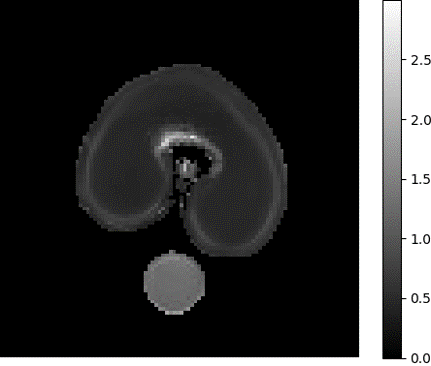
\includegraphics[width=0.9\textwidth]{fig/manualcorr_irm250_t2.png}
      \caption{}
      \label{subfig:manualcorr_irm250_t2.png}
    \end{subfigure}%
    \begin{subfigure}[c]{0.33\textwidth}
      \centering
      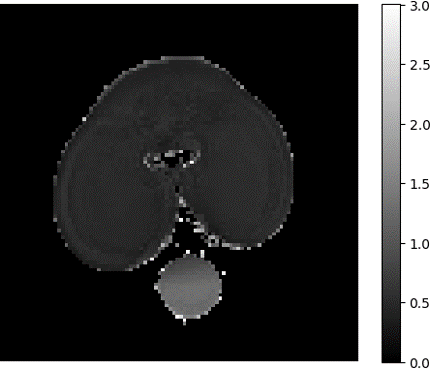
\includegraphics[width=0.9\textwidth]{fig/manualcorr_irm650_t2}
      \caption{}
      \label{subfig:manualcorr_irm650_t2}
    \end{subfigure}

    $\frac{\text{AX6}}{\text{AX5}}$  
    \begin{subfigure}[c]{0.66\textwidth}
      \centering
      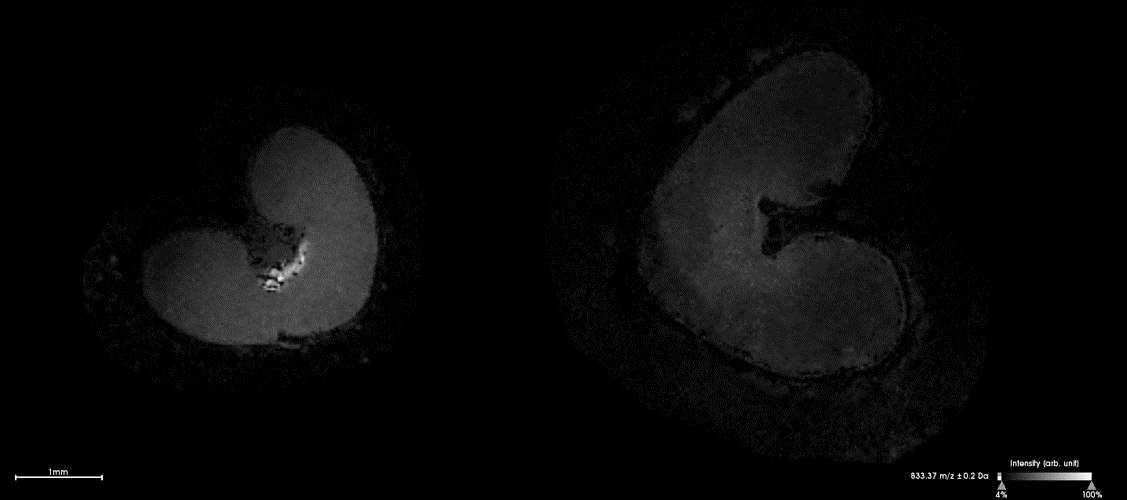
\includegraphics[width=0.8\textwidth]{fig/manualcorr_msi_250650}
      \caption{}
      \label{subfig:manualcorr_msi_250650}
    \end{subfigure}%
  \end{figure}
  

\end{frame}

\begin{frame}{Mise en corrélation manuelle}
   \begin{figure}[ht]
     \centering
     Densité
    \begin{subfigure}[c]{0.33\textwidth}
      \centering
      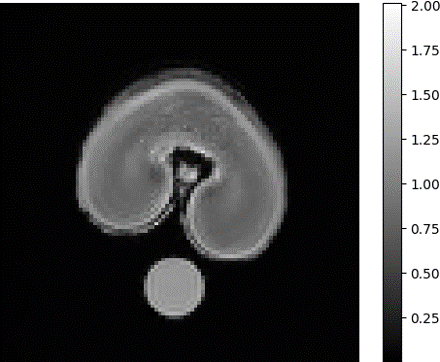
\includegraphics[width=0.9\textwidth]{fig/manualcorr_irm250_density.png}
      \caption{}
      \label{subfig:manualcorr_irm250_density.png}
    \end{subfigure}%
    \begin{subfigure}[c]{0.33\textwidth}
      \centering
      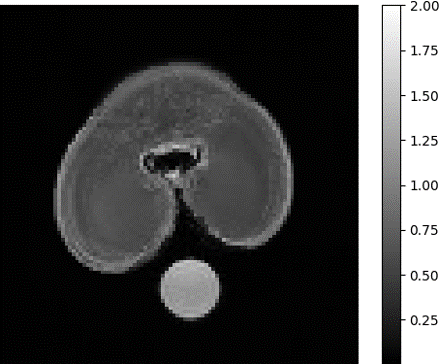
\includegraphics[width=0.9\textwidth]{fig/manualcorr_irm650_density}
      \caption{}
      \label{subfig:manualcorr_irm650_density}
    \end{subfigure}

    AX12 3.Ac
    \begin{subfigure}[c]{0.66\textwidth}
      \centering
      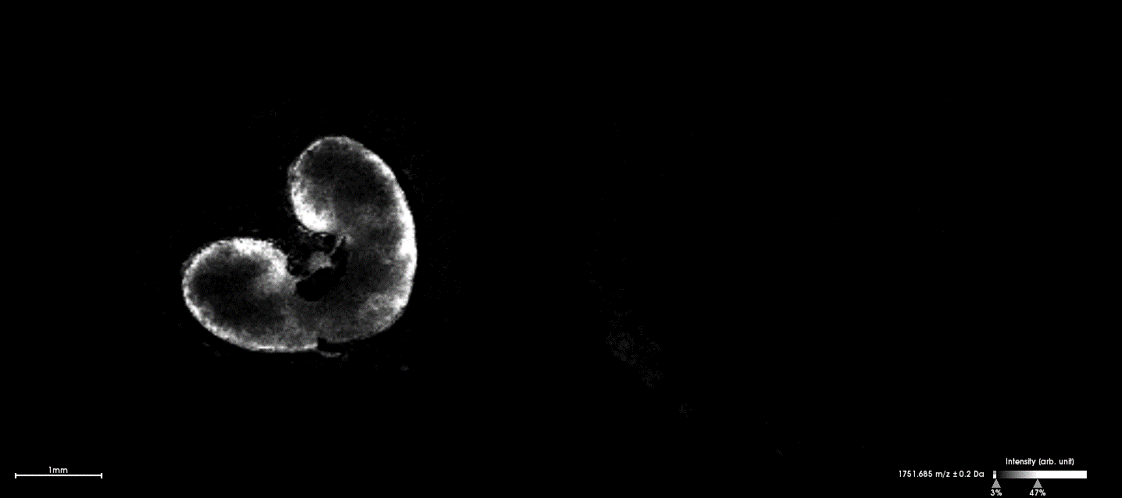
\includegraphics[width=0.8\textwidth]{fig/manualcorr_msi_250650_ac}
      \caption{}
      \label{subfig:manualcorr_msi_250650_ac}
    \end{subfigure}%
  \end{figure}
\end{frame}

\begin{frame}{Analyse statistique automatique}

  \begin{figure}
    \centering
    $T_2^*$
    \begin{subfigure}[c]{0.33\textwidth}
      \centering
      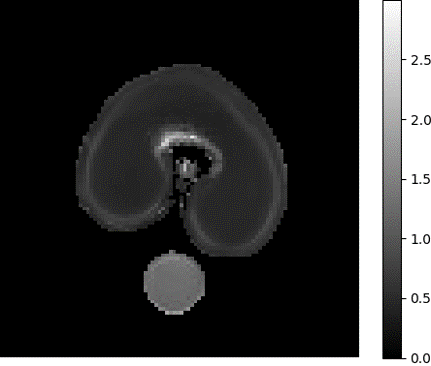
\includegraphics[width=0.9\textwidth]{fig/manualcorr_irm250_t2.png}
      \caption{}
      \label{subfig:manualcorr_irm250_t2.png}
    \end{subfigure}%
    \begin{subfigure}[c]{0.33\textwidth}
      \centering
      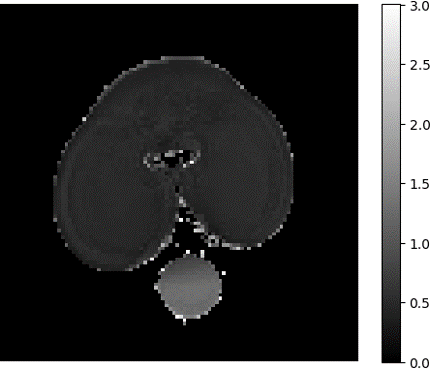
\includegraphics[width=0.9\textwidth]{fig/manualcorr_irm650_t2}
      \caption{}
      \label{subfig:manualcorr_irm650_t2}
    \end{subfigure}
    \begin{subfigure}[c]{0.33\textwidth}
      \centering
      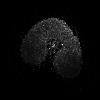
\includegraphics[width=0.8\textwidth]{fig/autocorr_msi_250}
      \caption{$\frac{833.33}{737.5}$}
      \label{subfig:autocorr_msi_250}
    \end{subfigure}%
    \begin{subfigure}[c]{0.33\textwidth}
      \centering
      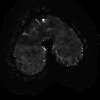
\includegraphics[width=0.8\textwidth]{fig/autocorr_msi_650}
      \caption{$\frac{1362.44}{835.34}$}
      \label{subfig:autocorr_msi_650}
    \end{subfigure}
  \end{figure}
  
\end{frame}

\begin{frame}{Analyse statistique automatique}

  \begin{figure}
    \centering
    Densité
    \begin{subfigure}[c]{0.33\textwidth}
      \centering
      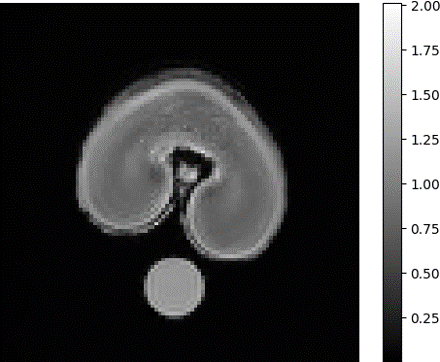
\includegraphics[width=0.9\textwidth]{fig/manualcorr_irm250_density.png}
      \caption{}
      \label{subfig:manualcorr_irm250_t2.png}
    \end{subfigure}%
    \begin{subfigure}[c]{0.33\textwidth}
      \centering
      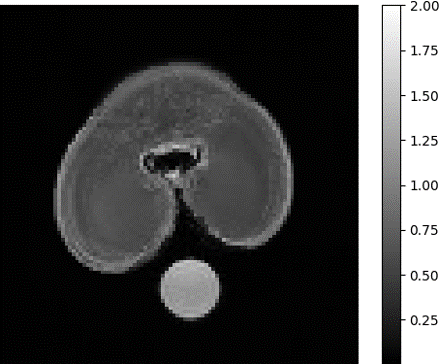
\includegraphics[width=0.9\textwidth]{fig/manualcorr_irm650_density}
      \caption{}
      \label{subfig:manualcorr_irm650_t2}
    \end{subfigure}
    \begin{subfigure}[c]{0.33\textwidth}
      \centering
      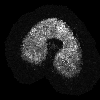
\includegraphics[width=0.8\textwidth]{fig/autocorr_msi_250_density}
      \caption{646.79}
      \label{subfig:autocorr_msi_250_density}
    \end{subfigure}%
    \begin{subfigure}[c]{0.33\textwidth}
      \centering
      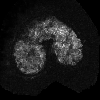
\includegraphics[width=0.8\textwidth]{fig/autocorr_msi_650_density}
      \caption{$\frac{835.34}{747.41}$}
      \label{subfig:autocorr_msi_650_density}
    \end{subfigure}
  \end{figure}
  
\end{frame}

\begin{frame}{Corrélations manuelles vs automatiques}
  Perception visuelle des images d'ions :
  \begin{itemize}
  \item<2-> \textbf{Zone de tir} ignorée
  \item<3-> \textbf{Bruit} ignoré
  \item<4-> Importance plus forte des zones où le \textbf{constraste varie}

  \end{itemize}

  \begin{figure}[ht]
    \centering
    \includegraphics<1>[width=0.9\textwidth]{fig/auto_1}%
    \includegraphics<2-3>[width=0.9\textwidth]{fig/auto_2}%
    \includegraphics<4->[width=0.9\textwidth]{fig/auto_3}
  \end{figure}


\end{frame}

\begin{frame}{Mise en corrélation automatique}

  \textbf{Objectif :} proposer une mise en corrélation automatique plus proche de la perception visuelle.

  \begin{enumerate}
  \item<1-> Zone de tir : \textbf{masque} utilisant l'image IRM
  \item<2-> Bruit : \textbf{filtres}
  \item<3-> Variations de contraste : \textbf{nouvelle mesure} statistique
  \end{enumerate}
\end{frame}


\begin{frame}{Masquage}
  Ignorer la zone de tir : \textbf{masquage} des régions où les intensités des pixels sont égales à 0 dans l'image IRM.

  \begin{figure}[ht]
    \centering
    \begin{subfigure}[t]{0.33\textwidth}
      \centering
      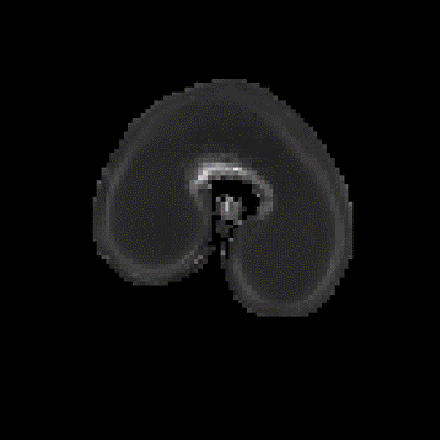
\includegraphics[width=0.9\textwidth]{fig/mri_slice8_250}
      \caption{}
      \label{subfig:mri_slice8_250}
    \end{subfigure}%
    \begin{subfigure}[t]{0.33\textwidth}
      \centering
      \includegraphics<1>[width=0.9\textwidth]{fig/zonetir_0}%
      \includegraphics<2>[width=0.9\textwidth]{fig/zonetir_1}%
      \includegraphics<3->[width=0.9\textwidth]{fig/zonetir_2}
      \caption{}
      \label{subfig:zonetir_0}
    \end{subfigure}%

  \end{figure}

  \visible<4-> {
    \textbf{Solution alternative : } seuil sur les faibles intensités dans les images d'ions.
  }
\end{frame}

\begin{frame}{Débruitage}
  \textbf{Débruitage :}
  \begin{itemize}
  \item Filtre \textbf{médian}
  \item Filtre gaussien
  \item Méthodes non-locales
  \end{itemize}

 \alert{Filtre médian} : bon compromis pour \textbf{préserver les détails} et \textbf{supprimer le bruit}.

 \begin{figure}[ht]
   \centering
   \begin{subfigure}[t]{0.33\textwidth}
     \centering
     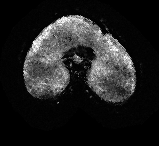
\includegraphics[width=0.9\textwidth]{fig/before_median}
     \caption{}
     \label{subfig:before_median}
   \end{subfigure}%
   \begin{subfigure}[t]{0.33\textwidth}
     \centering
     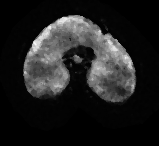
\includegraphics[width=0.9\textwidth]{fig/after_median}
     \caption{}
     \label{subfig:after_median}
   \end{subfigure}%

 \end{figure}


\end{frame}



\begin{frame}{Mesures spatiales}
  \textbf{Correspondances :} mesures dans l'espace réduit de la NMF.

  \textbf{Problème :} difficile d'analyser localement les correspondances spatiales.
  
  $\Rightarrow$ utilisation de la \textbf{similarité cosinus}.

  \alert{Similarité cosinus :} mesure la corrélation entre les intensités de deux images.
\end{frame}

\begin{frame}{Similarité cosinus}
  Peut s'assimiler à la \textbf{moyenne des différences d'intensités au carré} :

   \begin{figure}[ht]
    \centering
    \begin{subfigure}[t]{0.33\textwidth}
      \centering
      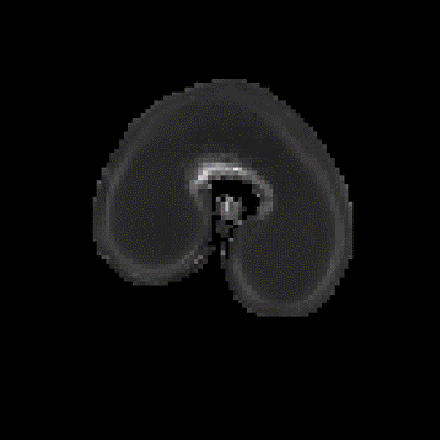
\includegraphics[width=0.9\textwidth]{fig/mri_slice8_250}
      \caption{}
      \label{subfig:mri_slice8_250}
    \end{subfigure}%
    \begin{subfigure}[t]{0.33\textwidth}
      \centering
      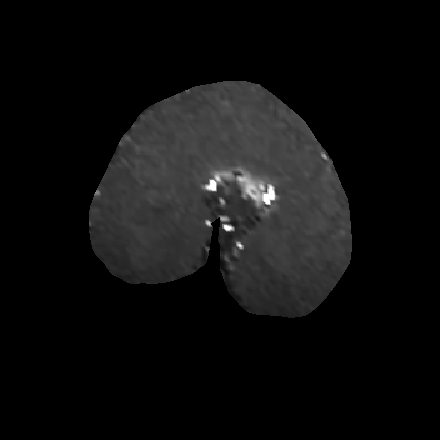
\includegraphics[width=0.9\textwidth]{fig/zonetir_2}%
      \caption{}
      \label{subfig:zonetir_0}
    \end{subfigure}%
    \begin{subfigure}[t]{0.33\textwidth}
      \centering
      \includegraphics<2>[width=0.9\textwidth]{fig/diff}%
      \includegraphics<3>[width=0.9\textwidth]{fig/diff_norm_sq}
      \visible<2->{
        \caption{\only<2>{Différences}\only<3>{Différences au carré}}
      }
    \end{subfigure}%

  \end{figure}
  
  
\end{frame}

\begin{frame}{Similarité cosinus}

  \textbf{Problème :} cette mesure favorise les régions d'intensités proches et de \textbf{grande taille}.

  \textbf{Exemple :} image d'ion avec la meilleure corrélation :
  
  \visible<2-> {
    \begin{figure}[ht]
      \centering
      \begin{subfigure}[t]{0.33\textwidth}
        \centering
        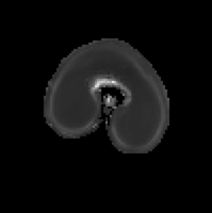
\includegraphics[width=0.9\textwidth]{fig/cosine_mri}
        \caption{}
        \label{subfig:cosine_mri}
      \end{subfigure}%
      \begin{subfigure}[t]{0.33\textwidth}
        \centering
        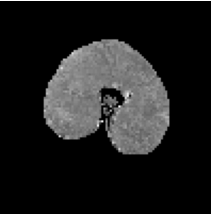
\includegraphics[width=0.9\textwidth]{fig/cosine_msi}%
        \caption{$\frac{1097.44}{965.38}$}
        \label{subfig:cosine_msi}
      \end{subfigure}%
      \begin{subfigure}[t]{0.33\textwidth}
        \centering
        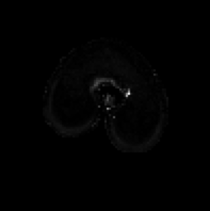
\includegraphics[width=0.9\textwidth]{fig/cosine_diff}%
        \caption{Différences au carré}
      \end{subfigure}%
    \end{figure}
  }
  

\end{frame}

\begin{frame}{Similarité cosinus pondérée}

  \textbf{Objectif :} donner plus d'importance aux pixels associés aux régions où le constraste varie.

  Pondération de la similarité cosinus par les gradients de l'image IRM :

  \begin{figure}[ht]
    \centering
    \begin{subfigure}[t]{0.33\textwidth}
      \centering
      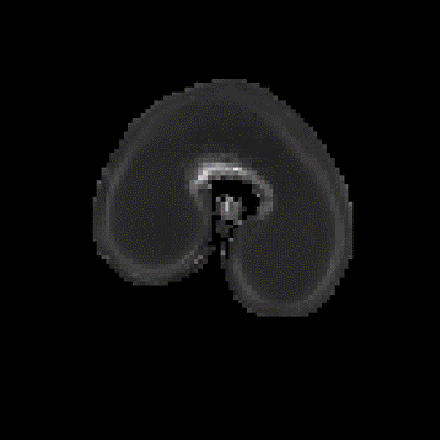
\includegraphics[width=0.9\textwidth]{fig/mri_slice8_250}
      \caption{}
      \label{subfig:mri_slice8_250}
    \end{subfigure}%
    \begin{subfigure}[t]{0.33\textwidth}
      \centering
      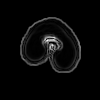
\includegraphics[width=0.9\textwidth]{fig/mri_slice8_sobel}
      \caption{Gradients}
      \label{subfig:mri_slice8_sobel}
    \end{subfigure}%
    \begin{subfigure}[t]{0.33\textwidth}
      \centering
      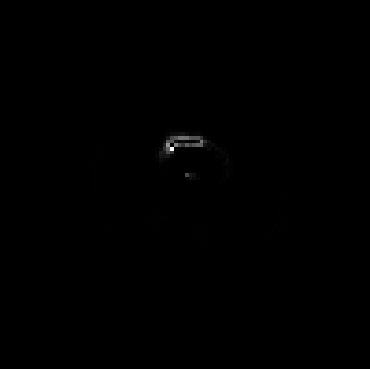
\includegraphics[width=0.9\textwidth]{fig/cosine_diffweight}
      \caption{Similarité pondérée}
      \label{subfig:cosine_diffweight}
    \end{subfigure}%

  \end{figure}


 
\end{frame}

\begin{frame}{Similarité cosinus pondérée}
  Résultats :

    \begin{figure}[ht]
    \centering
    \begin{subfigure}[t]{0.31\textwidth}
      \centering
      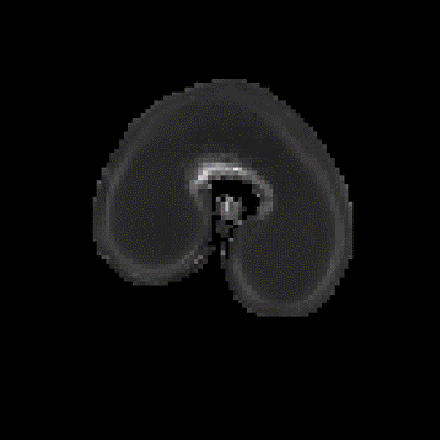
\includegraphics[width=0.9\textwidth]{fig/mri_slice8_250}
      \caption{}
      \label{subfig:mri_slice8_250}
    \end{subfigure}%
    \begin{subfigure}[t]{0.31\textwidth}
      \centering
      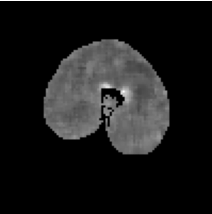
\includegraphics[width=0.9\textwidth]{fig/cosine_median}
      \caption{Filtre médian\\($\frac{714.06}{620.06}$)}
      \label{subfig:cosine_median}
    \end{subfigure}%
    \begin{subfigure}[t]{0.31\textwidth}
      \centering
      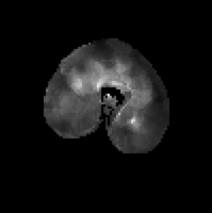
\includegraphics[width=0.9\textwidth]{fig/cosine_weight}
      \caption{Filtre médian + pondération\\($\frac{1404.34}{1181.42}$)}
      \label{subfig:cosine_weight}
    \end{subfigure}%

  \end{figure}
\end{frame}

\begin{frame}{Autres tentatives}

  

  \begin{itemize}
  \item Analyser chaque région indépendamment ($k$-means)
  \item  Autre mesure de similarité : \textbf{Universal Image Quality Index} (UIQ) \cite{Zhou_Wang_2002}.
    
  $\Rightarrow$ produit de 3 termes liés à : (a) la luminance, (b) le contraste et (c) la corrélation entre intensités.
\end{itemize}

    \begin{figure}[ht]
    \centering
    \begin{subfigure}[t]{0.31\textwidth}
      \centering
      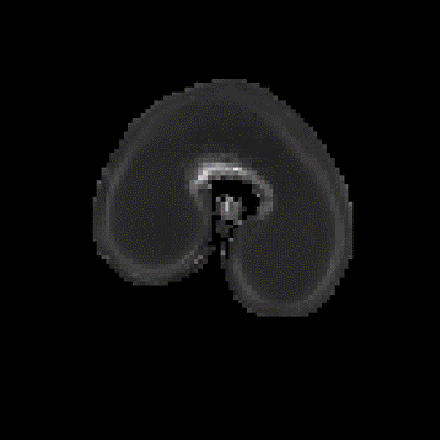
\includegraphics[width=0.9\textwidth]{fig/mri_slice8_250}
      \caption{}
      \label{subfig:mri_slice8_250}
    \end{subfigure}%
    \begin{subfigure}[t]{0.31\textwidth}
      \centering
      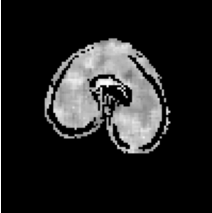
\includegraphics[width=0.9\textwidth]{fig/cosine_kmeans}
      \caption{$k$-means\\($\frac{1348.77}{885.1}$)}
      \label{subfig:cosine_kmeans}
    \end{subfigure}%
    \begin{subfigure}[t]{0.31\textwidth}
      \centering
      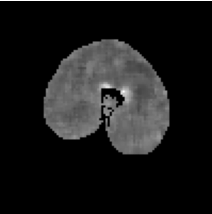
\includegraphics[width=0.9\textwidth]{fig/cosine_median}
      \caption{UIQ\\($\frac{714.06}{620.06}$)}
      \label{subfig:cosine_uiq}
    \end{subfigure}%

  \end{figure}
\end{frame}


\begin{frame}{Intégration à la NMF}
  Nouveaux traitements précédant l'analyse statistique :
  \begin{enumerate}
  \item Masquage
  \item Débruitage
  \item Pondération par les gradients (facultatif)
  \end{enumerate}

  Ici : \textbf{sans pondération}. Résultats avec pondération \textbf{en cours}.
\end{frame}


\begin{frame}{Stade 250DJ}
  De façon générale : corrélation apportée par les images \textbf{homogènes} en intensité.

  \begin{itemize}
  \item  $T_2^*$ : slices 9 et 11 (milieu-bas du grain) : rapport $\frac{\text{AX6}}{\text{AX5}}$ en tête.
  \item   Densité : slices 3 et 4 : rapports d'AX avec des degrés d'acétylation différents ($\frac{\text{AX7.3Ac}}{\text{AX5.6Ac}}$, $\frac{\text{AX6.2Ac}}{\text{AX6.1Ac}}$, ...)
  \end{itemize}


  \begin{figure}[ht]
    \centering
    \begin{subfigure}[t]{0.33\textwidth}
      \centering
      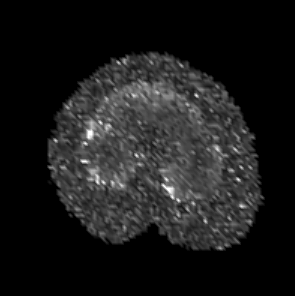
\includegraphics[width=0.9\textwidth]{fig/density_250_slice3}
      \caption{$\frac{\text{AX7.3Ac}}{\text{AX5.6Ac}}$}
      \label{subfig:density_250_slice3}
    \end{subfigure}%
    \begin{subfigure}[t]{0.33\textwidth}
      \centering
      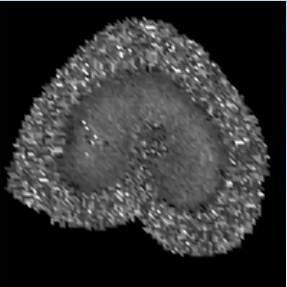
\includegraphics[width=0.9\textwidth]{fig/density_250_slice4}
      \caption{$\frac{\text{AX6.2Ac}}{\text{AX6.1Ac}}$}
      \label{subfig:density_250_slice4}
    \end{subfigure}%

  \end{figure}


\end{frame}


\begin{frame}{Stade 650DJ}
  De façon générale : corrélation apportée par les images \textbf{homogènes} en intensité.

   \begin{itemize}
  \item  $T_2^*$ : slices 6, 8, 9 : rapports sans Ac ($\frac{\text{AX7}}{\text{AX5}}$, $\frac{\text{AX9}}{\text{AX8}}$, ...)
  \item  Densité : slices 3, 7, 10 et 11 : rapports sans Ac ($\frac{\text{AX9}}{\text{AX8}}$, $\frac{\text{AX7}}{\text{AX6}}$,...)
  \end{itemize}

    \begin{figure}[ht]
      \centering
          \begin{subfigure}[t]{0.25\textwidth}
      \centering
      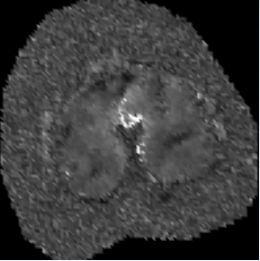
\includegraphics[width=0.9\textwidth]{fig/t2_650_slice6}
      \caption{$\frac{\text{AX7}}{\text{AX5}}$}
      \label{subfig:density_650_slice10}
    \end{subfigure}%
    \begin{subfigure}[t]{0.25\textwidth}
      \centering
      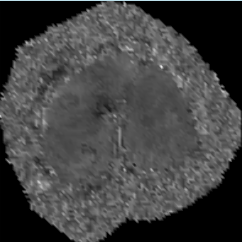
\includegraphics[width=0.9\textwidth]{fig/t2_650_slice8}
      \caption{$\frac{\text{AX9}}{\text{AX8}}$}
      \label{subfig:density_650_slice11}
    \end{subfigure}%
    \vrule%
    \begin{subfigure}[t]{0.25\textwidth}
      \centering
      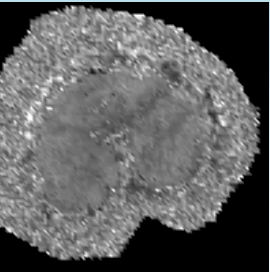
\includegraphics[width=0.9\textwidth]{fig/density_650_slice10}
      \caption{$\frac{\text{AX9}}{\text{AX8}}$}
      \label{subfig:density_650_slice10}
    \end{subfigure}%
    \begin{subfigure}[t]{0.25\textwidth}
      \centering
      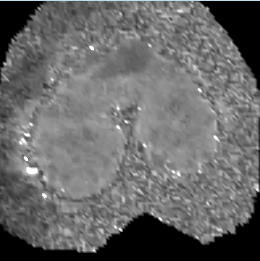
\includegraphics[width=0.9\textwidth]{fig/density_650_slice11}
      \caption{$\frac{\text{AX7}}{\text{AX6}}$}
      \label{subfig:density_650_slice11}
    \end{subfigure}%

  \end{figure}
\end{frame}




\AtBeginSection[]{
  \begingroup
  \setbeamercolor{background canvas}{bg=mLightBlue}
  
  \setbeamertemplate{subsection in toc}
  {\leavevmode\leftskip=2em$\bullet$\hskip1em\inserttocsubsection\par}
  \setbeamercolor{section in toc}{fg=paleGrey, bg=mLightBlue}
  \setbeamercolor{local structure}{fg=mLightBlueLighter,bg=mLightBlue}
  \setbeamercolor{section in toc shaded}{fg=mLightBlue, bg=mLightBlue}
  \setbeamertemplate{section in toc}[circle]
  \setbeamertemplate{section in toc shaded}[default][80]
  \setbeamertemplate{section in toc}{\hspace*{1em}\inserttocsection}

  \setbeamercolor{subsection in toc}{fg=paleGrey, bg=mLightBlue}
  \begin{frame}[noframenumbering,plain]
    \frametitle{\textcolor{paleGrey}{Table des matières}}

    \tableofcontents[currentsection, sectionstyle=show/hide, hideothersubsections]
  \end{frame}
  \endgroup
}



\section{Plan de publication}

\begin{frame}{Plan de publication}

  Nouveaux résultats:
  \begin{itemize}
  \item<2-> Qui porte la publication?
  \item<3-> Que manque-t-il d'un point de vue expérimental?
  \item<4-> Autre publication méthodo envisageable? 
  \end{itemize}


\end{frame}


\nocite{*}

\appendix
\setbeamertemplate{headline}{%
  % \nointerlineskip
  % \begin{beamercolorbox}[wd=\paperwidth,leftskip=0.5cm,ht=0pt,dp=0pt]{block title}%
  %   \usebeamerfont{page number in head/foot}{\insertsection}
  % \end{beamercolorbox}%
  % \if@useTitleProgressBar
  % \nointerlineskip
  % % \vspace{-0.7cm}
  % \begin{beamercolorbox}[wd=\paperwidth,ht=0pt,dp=5pt]{section}
  %   \progressbar@titleprogressbar
  % \end{beamercolorbox}
  % \fi
  % \nointerlineskip
}

% \setbeamertemplate{frametitle}{%
%   \begin{beamercolorbox}[wd=\paperwidth,leftskip=0.7cm,rightskip=0.3cm,ht=0pt,dp=0pt]{frametitle}
%     \usebeamerfont{frametitle}\MakeLowercase{\protect\insertframetitle}
%   \end{beamercolorbox}
% }

\begin{frame}[allowframebreaks]
  \frametitle{Références}
  \setbeamertemplate{bibliography item}{$\bullet$}
  \bibliographystyle{apalike}
  \scriptsize{
    \bibliography{main}
  }
\end{frame}


\end{document}
